%%%%%%%%%%%%%%%%%%%%%%%%%%%%%%%%%%%%%%%%%%%%%%%%%%%%%%%%%%%%%%%%%%%%%%%%%%%%%%%%%%
%%% Control
%%%
%%% NEED TO FIX NOTATIONS
%%%
%%%%%%%%%%%%%%%%%%%%%%%%%%%%%%%%%%%%%%%%%%%%%%%%%%%%%%%%%%%%%%%%%%%%%%%%%%%%%%%%%%
\chapter{System Modeling}
	\label{ch::system_modeling}

	%Analysis and control of the BlueFoot quadruped requires the utilization of both kinematic and dynamical system models.
	
	\section{Kinematic Model}
		\label{sec::system_kinematics}

		The kinematic model of the BlueFoot platform is paramount for trajectory planning, localization, and adaptation in the robot task-space. In particular, inverse position and velocity solutions are used to prescribe joint-space commands from particular foot trajectories planned in the world coordinate frame. Additionally, BlueFoot's forward kinematic model is utilized to estimate the position of each foot using the position and orientation of the trunk; and joint position feedback. This section will describe BlueFoot's forward and inverse kinematic models, as well as how these models are used in motion planning and control tasks.

		\subsection{Forward Position Kinematics}
			\label{ch::system_modeling_pos_kin}

			To formulate the kinematics model, a set of coordinate systems have been defined and are described by Figure~\ref{fig::coordinate_frames}. Note that the frame $O_{0}$ represents the world coordinate frame; and $O_{b}$ is the coordinate frame, centered at  ${p}_{b}$ attached to the platform and is always aligned with $O_{0}$. $O_{b}$ represents a body frame rigidly attached to the center of the trunk. The orientation and position of the trunk are defined by vectors of $\theta_{b}\InRe{3}$ and ${p}_{b}\InRe{3}$, which relate the frame $O_{b}$ to the world frame $O_{0}$. Coordinate frames $O_{i,0}$ are attached to the first joint of each \Ith leg.
%
				\begin{figure}[h!]
					\centering
					\fbox{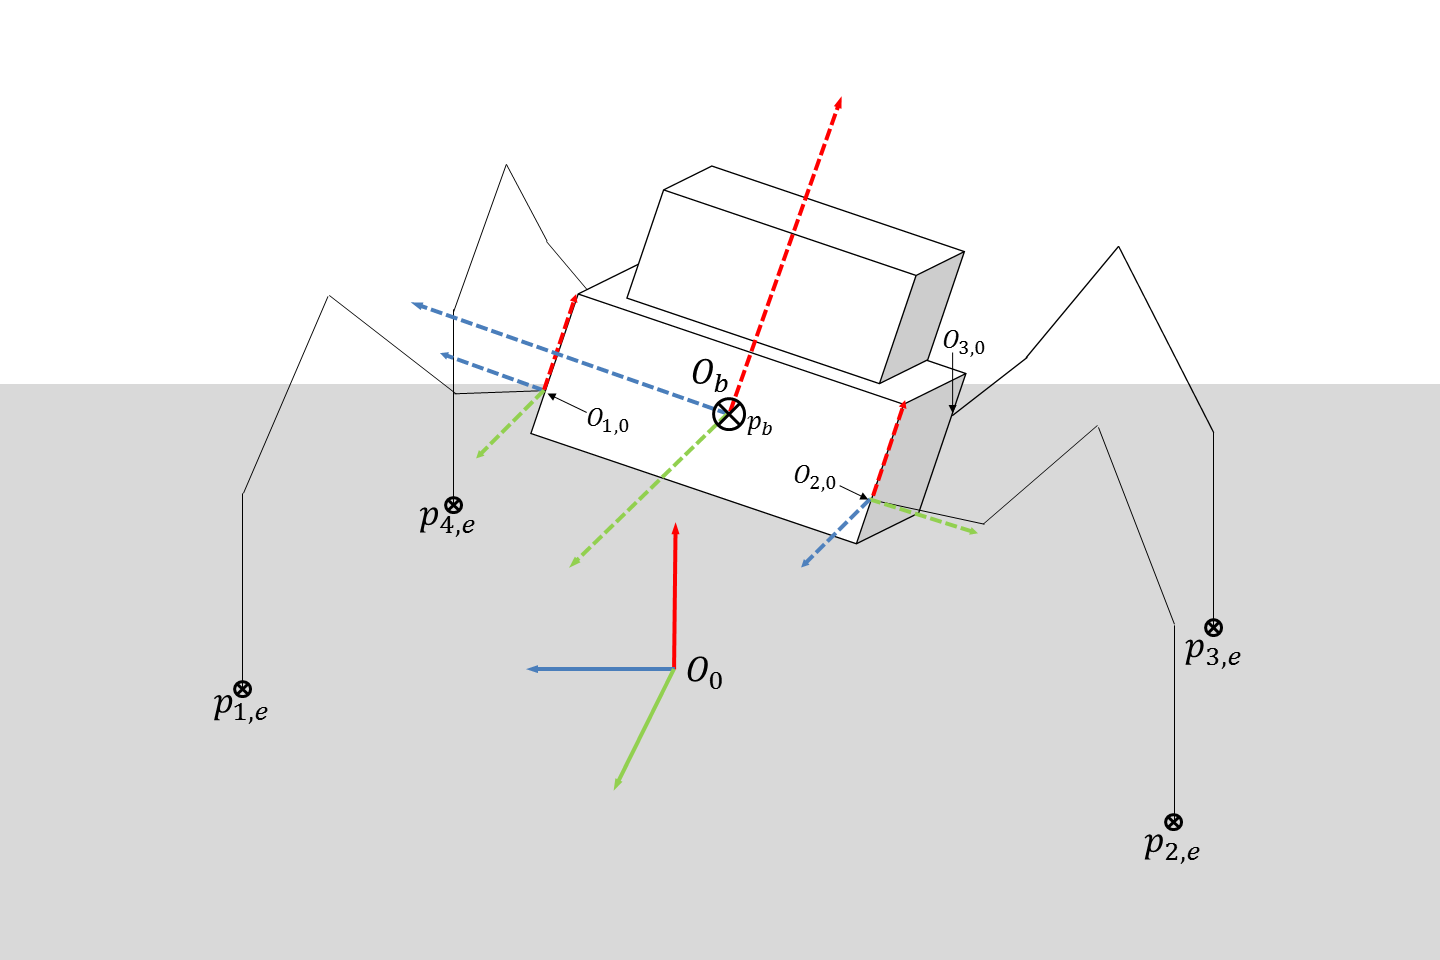
\includegraphics[width=1.00\textwidth]{coordinate_frames.png}}
					\caption{A visualization of BlueFoot's coordinate frame configuration.}
					\label{fig::coordinate_frames}
				\end{figure}
%
			The \Jth joint position of each \Ith leg is represented  by the points ${p}_{i,j}$ in the frame $O_{0}$. These spatial locations are generated from a combination of the body orientation, $\theta_{b}$, and joint positions for each \Ith leg, $q_{i} = [q_{i,1}, q_{i,2}, q_{i,3}, q_{i,4}]^T$. $q_{i,1}$ represents the position of the hip-joint (joint closest to the center platform), which rotates in the direction of the transverse body plane. The joint variables $q_{i,2}, q_{i,3}$ and $q_{i,4}$ represent the lateral-hip, knee and ankle joint rotations, respectively.

			The coordinate transformation between world coordinate frame, $O_{0}$, and the zeroth Denavit-Hartenberg (DH) coordinate frame of leg \emph{i}, $O_{i,0}$ (located at the origin of joint-1), is given by
				\begin{equation}
					H_{0}^{i,0} = \left[ 
					\begin{array}{c|c}
						R_{zyx}(\theta_{b}) R_{z}(\sigma_{i})	&R_{zyx}(\theta_{b}) \nu + {p}_{b} 	\\ \hline
						0										&	1											\\
					\end{array} 
					\right]
					\label{eq::world_to_dh}
				\end{equation}
			where $\sigma_{i} \equiv \frac{\pi}{2}(i-1) + \frac{\pi}{4} $ and $\nu \equiv  R_{z}(\sigma_{i}) \beta$ with $\beta$ defining an offset from $O_{b}$ to where the first joint of each leg is attached to the body. $R_{zyx}$ represents a rotation associated with the pitch (x-axis), roll (y-axis), and yaw (z-axis) angles of the main body about the platform frame, $\theta_{b}$. $R_{z}$ represents a rotation about the (z-axis) of the frame $O_{b}$. 

			A transformation from the zeroth DH frame of the to the $(j+1)^{th}$ joint of leg \emph{i} is described, in general, by
				\begin{equation}
					H^{i,0}_{i,j} =
					\left[ 
					\begin{array}{c|c}
						R^{i,0}_{i,j} 	&	{p}^{i,0}_{i,j} 	\\ \hline
						0			&	1				\\
					\end{array} 
					\right].
				\end{equation}

			The kinematics of each leg are identical. Thus, the transformations $H^{i,0}_{i,j}$ are of the same form and are derived by the DH parameters given by Table \ref{tab::dh_params}. Actual values for the link lengths $a_{1-4}$ and body-offset, $\nu$, are provided in Table \ref{tab::link_lens}.


			\begin{table}[h]
				\centering
				\begin{tabularx}{150mm}{|C{0.2}|C{0.2}|C{0.2}|C{0.2}|C{0.2}|} \hline
					\textbf{Link}	&\textbf{$a_i$} &	\textbf{$\alpha_i$}	&	\textbf{$d_i$}	&	\textbf{$\theta_i$} \\ \hline \hline
					1				&	$a_{1}$		&	$\pi/2$				&	0				&	$q_{i,1}^*$			\\ \hline
					2				&	$a_{2}$		&	0					&	0				&	$q_{i,2}^*$			\\ \hline
					3				&	$a_{3}$		&	0					&	0				&	$q_{i,3}^*$			\\ \hline
					4 				&	$a_{4}$		&	0					&	0				&	$q_{i,4}^*$			\\ \hline
				\end{tabularx}
				\caption{DH parameters for all legs.}
				\label{tab::dh_params}
			\end{table}
			

			Using these DH parameters, the transformations $H^{i,0}_{i,1}$, $H^{i,0}_{i,2}$, $H^{i,0}_{i,3}$, and $H^{i,0}_{i,4}$ can be computed explicitly as follows:
				%% Manipulator Base to Frame 1 %%
				\begin{equation} 
					H^{i,0}_{i,1} =\left[ 
					\begin{array}{ccc|c}
						c_{1,i} 	&  		0	& 	s_{1,i}		&		c_{1,i} a_{1,i}	\\
						s_{1,i} 	&  		0	& 	-c_{1,i}	&		s_{1,i} a_{1,i}	\\
						0 			&  		1	& 	0			&		0 				\\ \hline
						0 			&  		0	& 	0			&		1 				\\
					\end{array} 
					\right]
				\end{equation}
				%% Manipulator Base to Frame 2 %%
				\begin{equation}
					H^{i,0}_{i,2} =\left[ 
					\begin{array}{ccc|c}
						c_{1,i} c_{2,i}	&  		-c_{1,i} s_{2,i}	& 		s_{1,i}		&	c_{1,i}( a_{1,i} + a_2 c_{2,i} )\\
						s_{1,i} c_{2,i}	&  		-s_{1,i} s_{2,i}	& 		-c_{1,i}	&	s_{1,i}( a_{1,i} + a_2 c_{2,i} )\\
						s_{2,i} 		&  		c_{2,i}			 	& 		0			&	a_2 s_{2,i} 					\\ \hline
						0 			&  		0			 		& 		0			&	1 								\\
					\end{array} 
					\right]
				\end{equation}
				%% Manipulator Base to Frame 3 %%
				\begin{equation}
					H^{i,0}_{i,3} =\left[ 
					\begin{array}{ccc|c}
						c_{1,i} c_{23,i}	&  		-c_{1,i} s_{23,i}	& 		s_{1,i}		&		c_{1,i}( a_{1,i} + a_2 c_{2,i} + a_3 c_{23,i} )	\\
						s_{1,i} c_{23,i}	&  		-s_{1,i} s_{23,i}	& 		-c_{1,i}	&		s_{1,i}( a_{1,i} + a_2 c_{2,i} + a_3 c_{23,i} )	\\
						s_{23,i} 		&  		c_{23,i}			& 		0			&		a_2 s_{2,i} + a_{3,i} s_{23,i}			\\ \hline
						0 			&  		0					& 		0			&		1 										\\
					\end{array} 
					\right]
				\end{equation}
				%% Manipulator Base to Frame 4 %%
				\begin{equation}
					H^{i,0}_{i,4} =\left[ 
					\begin{array}{ccc|c}
						c_{1,i} c_{234,i}	&  		-c_{1,i} s_{234,i}	& 		s_{1,i}		&		c_{1,i}( a_{1,i} + a_2 c_{2,i} + a_3 c_{23,i} + a_4 c_{234,i} )		\\
						s_{1,i} c_{234,i}	&  		-s_{1,i} s_{234,i}	& 		-c_{1,i}	&		s_{1,i}( a_{1,i} + a_2 c_{2,i} + a_3 c_{23,i} + a_4 c_{234,i} )		\\
						s_{234,i} 		&  		c_{234,i}		& 		0			&		a_2 s_{2,i} + a_3 s_{23,i} + a_4 s_{234,i}					\\ \hline
						0 			& 		0			& 		0			&		1 															\\
					\end{array} 
					\right]
				\end{equation}

			The position of joint 1 of leg \emph{i} in $O_{0}$, ${p}_{i,1}$ may now be computed with respect to frame $O_{0}$ by:
				\begin{equation}
					{p}_{i,1} \equiv E_{p} H_{0}^{i,0} e_{p}.
					\label{eq::world_joint1_position}
				\end{equation}
			where
				\begin{eqnarray}
					E_{p} = [I_{3\times3},0_{3\times1}]	\nonumber 	\\
					e_{p} = [0_{1\times3},1]^T.			\nonumber 	
				\end{eqnarray}
			The position of joints 2-4 of leg \emph{i}, may now be computed with respect to frame $O_{0}$ by:
				\begin{equation}
					{p}_{i,j} \equiv E_{p} H_{0}^{i,0} {H}^{i,0}_{i,(j-1)} e_{p}. \Sep \forall \Sep j\in\{2,3,4\}
					\label{eq::world_joint_positions}
				\end{equation}
			Finally, the position of the end-effector (foot) of \Ith leg. ${p}_{i,e}$, is achieved as follows:
				\begin{equation}
					{p}_{i,e} \equiv E_{p} H_{0}^{i,0} {H}^{i,0}_{i,4} e_{p}.
					\label{eq::world_feet_positions}
				\end{equation}
			As a previously mentioned, BlueFoot's forward kinematic solution is used most prevalently in the estimating the position of each foot. Given estimates for body position and orientation, $\hat{p}_{b}$ and $\hat{\theta}_{b}$, a foot position estimate is explicitly define as a random variable:
				\begin{equation}
					\hat{p}_{i,e} = {p}_{i,e} + \Delta {p}_{i,e}
					\label{eq::foot_position_esitmate}
				\end{equation}
			where $\Delta {p}_{i,e}$ is a random error which arises from variations due to noise in sensed joint positions, as well as error in the estimates $\hat{p}_{b}$ and $\hat{\theta}_{b}$.


			\subsubsection{A Note about Foot Localization in the Robot-Relative Frames}

			Using the previously defined forward kinematics model and the relationships defined in \ref{eq::world_joint_positions} and \ref{eq::world_feet_positions}, the position of each joint and foot can be computed assuming the $p_{b}$ and $\theta_{b}$ are known (or can be estimated) in the frame $O_{0}$. Provided inertial feedback, trunk orientation, $\theta_{b}$, can be estimated by the use of an Extended Kalman Filter (EKF). $p_{b}$, however, requires more sophisticated localization measures, such as a Simultaneous Localization and Mapping (SLAM) scheme or absolute positioning via overhead camera or GPS. In lieu of an implementation for such a localization routine, it is convenient to generate foot positions estimate in a \emph{robot-relative} frame, $O_{b^{'}}$. This frame is not rigidly attached to the robot but moves along with the robot in $O_{0}$ according to the commanded translational velocity, $v^{r}$, and turning rate. $\omega^{r}$, administered to navigate the system. These values will be described in more detail in Chapter~\ref{ch::navigation}. Moreover, this frame has its own position relative to $O_{0}$, defined by the translation $p_{0}^{b'}$. $O_{b^{'}}$ is constantly aligned to $O_{0}$, with respect to rotation, making the rotation matrix which relates $O_{b^{'}}$ to $O_{0}$ the identity matrix.

			In this frame, the trunk position is regarded as an offset from the origin of $O_{b^{'}}$, $p_{b}^{b'}$. Since there is zero rotation between $O_{0}$ and $O_{b^{'}}$, the trunk rotation vector $\theta_{b}^{b'}$ is directly equivalent to $\theta_{b}$ in $O_{0}$. Using these translation and rotation definitions in place of their world frame counterparts, the robot-relative joint and foot-positions, ${p}_{i,j}^{b'}$ and ${p}_{i,e}^{b'}$ of each \Ith leg can be computed by defining a transformation from the robot relative frame to the first DH-frame for each leg, as follows:
				\begin{equation}
					H_{b^{'}}^{i,0} = 
					\left[ 
					\begin{array}{c|c}
						R_{zyx}(\theta_{b}) R_{z}(\sigma_{i})	&R_{zyx}(\theta_{b}) \nu + {p}_{b}^{b'} 	\\ \hline
						0										&	1												\\
					\end{array} 
					\right]
					\label{eq::rr_to_dh}
				\end{equation}
			which follows the same definitions in \ref{eq::world_to_dh}. The transformation defined in \ref{eq::rr_to_dh} is used as a direct replacement for the matrix $H_{0}^{i,0}$ in \ref{eq::world_joint_positions} and \ref{eq::world_feet_positions} in computing the corresponding positions, ${p}_{i,j}^{b'}$ and ${p}_{i,e}^{b'}$. Knowledge of these positions is useful for planning foot and body-placement which depend directly on the location relative foot and body positions, but do not necessarily depend on the position of the robot in the world coordinate frame.
 

		\subsection{Inverse Position Kinematics}
			\label{sec::inverse_position_kinematics}
			
			A foot configuration is specified by its coordinates ${p}_{e}$ and an ankle orientation, $\gamma_{i}$,  which represents a rotation about the axis of rotation of the second joint (lateral hip). Given a desired platform configuration, $\{ {p}_{b}, \theta_{b} \}$,  and desired \Ith foot configuration,  $\{ {p}_{i,e} , \gamma_{i} \}$, the inverse kinematics solution for each \Ith leg, ${q}_{i}$, is derived to be:

				\begin{eqnarray}
					q_{i,1} &=& \cos(i\pi) \wrap{ \frac{\pi}{4} - \psi_{i} } \nonumber\\
					q_{i,2} &=&	\tan^{-1} \wrap{\frac{\zeta_{i,z}}{\sqrt{\zeta_{i,x}^2+\zeta_{i,y}^2}}} \mp \cos^{-1}\wrap{\frac{a_{3}^2-a_{2}^2-\norm{\zeta_{i}}^2}{2 a_{2} \norm{\zeta_{i}} }} \pm \pi 	\nonumber\\
					q_{i,3} &=&	\mp \cos^{-1}\frac{\norm{\zeta}^2-a_{2}^2-a_{3}^2}{2 a_{2} a_{3}} \nonumber\\
					q_{i,4} &=&	\gamma_{i} - q_{i,2} - q_{i,3}	
				\end{eqnarray}
				%
				%
				where
				%
				%
				\begin{eqnarray}
					{p}_{i,e}^{i,0} &=&
					E_{p} 
					\wrap{ {H}_{i,k}^{0} } ^{-1}
					\left[
						\begin{array}{c}
							{p}_{i,e} 		\\
							1 				\\ 	
						\end{array}
					\right]	\nonumber\\																						\nonumber\\
					\psi_{i} 	&\equiv&	\tan^{-1}\wrap{ \frac{\ycomp{{p}_{i,e}^{i,0}}}{\xcomp{{p}_{i,e}^{i,0}} } }												\nonumber\\
					\zeta_{i,x} &\equiv& 	\ycomp{{p}_{i,e}^{i,0}} \sin(\psi_{i}) + \xcomp{{p}_{i,e}^{i,0}} \cos(\psi_{i}) - a_{4} \cos(\gamma_{i}) - a_{1} 						\nonumber\\
					\zeta_{i,y} &\equiv& 	\ycomp{{p}_{i,e}^{i,0}} \cos(\psi_{i}) - \xcomp{{p}_{i,e}^{i,0}} \sin(\psi_{i}) 											\nonumber\\
					\zeta_{i,z}	&\equiv&  	\zcomp{{p}_{i,e}^{i,0}} - a_{4} \sin(\gamma_{i}) .
				\end{eqnarray}
			Here, ${p}_{i,e}^{i,0}$ represents the position of each \Ith foot with respect to the zeroth DH frame of each \Ith leg; and $\xcomp{{p}_{i,e}^{i,0}}$, $\ycomp{{p}_{i,e}^{i,0}}$ and $\zcomp{{p}_{i,e}^{i,0}}$ represent the $x$, $y$, and $z$ axis coordinates of the vector ${p}_{i,e}^{i,0}$. The selection matrix $E_{p}$ is defined as it is in \ref{eq::world_joint1_position}-\ref{eq::world_feet_positions}.

			It is important to note that the ankle specification,  $\gamma_{i}$, adds extra constraints on the system kinematics and, thus, reduces the number of inverse kinematics solutions per foot position to two.


		\subsubsection{Range of Motion}

			The range of articulation of BlueFoot's main body has been characterized with respect to a set of imposed joint limits (see Table \ref{tab::JointLimits}) and has been performed with all feet fixed in a default stance (see Table \ref{tab::DefaultStance}). These limits have been selected according to the range of feasible angular position outputs of inverse position kinematics solution.
			\begin{table}[h]
				\centering
				\begin{tabularx}{\textwidth}{|C{0.25}|C{0.1875}|C{0.1875}|C{0.1875}|C{0.1875}|} \hline
					Joint Var.	&	${\theta_{i,1}}_{}$, rad		&		${\theta_{i,2}}_{}$, rad		&		${\theta_{i,3}}_{}$, rad		&		${\theta_{i,4}}_{}$, rad 	\\ \hline \hline
					Max Range	&	45$^o$				&		90$^o$				&		90$^o$				&		90$^o$			\\ \hline
					Min Range	&  -45$^o$				&	   -90$^o$				&	   -90$^o$				&	   -90$^o$			\\ \hline
				\end{tabularx}
				\caption{Imposed joint limits.}
				\label{tab::JointLimits}
			\end{table}
			
			It should be noted that the imposed joint limits are soft limits that have been chosen because of the
			typical range of motion executed by each joint during locomotion. Physical joint limits are tabulated in Table \ref{tab::HardJointLimits}.
			\begin{table}[h]
				\centering
				\begin{tabularx}{\textwidth}{|C{0.25}|C{0.1875}|C{0.1875}|C{0.1875}|C{0.1875}|} \hline
					Joint Var.	&	${q_{i,1}}_{}$, rad					&		${q_{i,2}}_{}$, rad		&		${q_{i,3}}_{}$, rad		&		${q_{i,4}}_{}$, rad 	\\ \hline \hline
					Max Range	&	82$^o$				&	102$^o$				&	102$^o$								&	102$^o$				\\ \hline
					Min Range	&  -69$^o$				&	-102$^o$			&	-102$^o$							&	-102$^o$			\\ \hline
				\end{tabularx}
				\caption{Physical joint limits.}
				\label{tab::HardJointLimits}
			\end{table}
			\begin{table}[h]
				\centering
				\begin{tabularx}{\textwidth}{|C{0.25}|C{0.15}|C{0.15}|C{0.15}|C{0.15}|C{0.15}|} \hline
							& 	$p_{b}^{b'}$	&	$p_{1,e}^{b'}$ 	& 	$p_{2,e}^{b'}$ 	&	$p_{3,e}^{b'}$	&	$p_{4,e}^{b'}$ 	\\ \hline \hline
					x (m)	&	*			&	 	0.165	&	-0.165		&	-0.165		&	0.165		\\ \hline
					y (m)	&	*			&		0.165	&	0.165		&	-0.165		&	-0.165		\\ \hline
					z (m)	&	0.115		&		 0		&		0		&		0		&	0			\\ \hline
				\end{tabularx}
				\caption{Locations for the platform and feet when in the default stance, written with respect to the frame $O_{b'}$.}
				\label{tab::DefaultStance}
			\end{table}

			Figures \ref{fig::pos_and_ori_rom} depicts the maximum pitch and roll and region of planar motion that the main body can reach while in the default stance. The blue shaded region of each figure (labeled \emph{Region of Failure}) depicts points at which joint positions exceed the imposed limits.
			\begin{figure}[h!]
				\centering
				\fbox{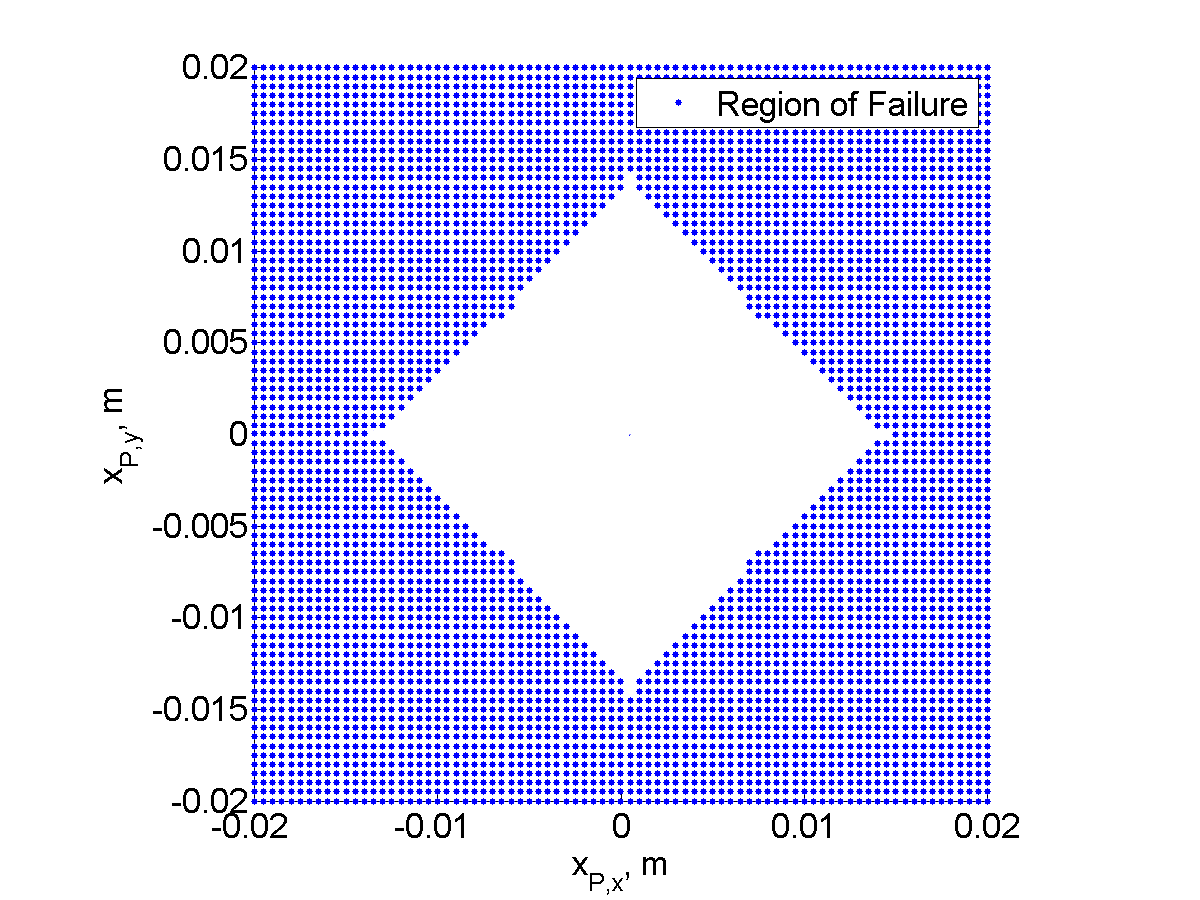
\includegraphics[width=0.495\textwidth]{pos_rom.png}}
				\fbox{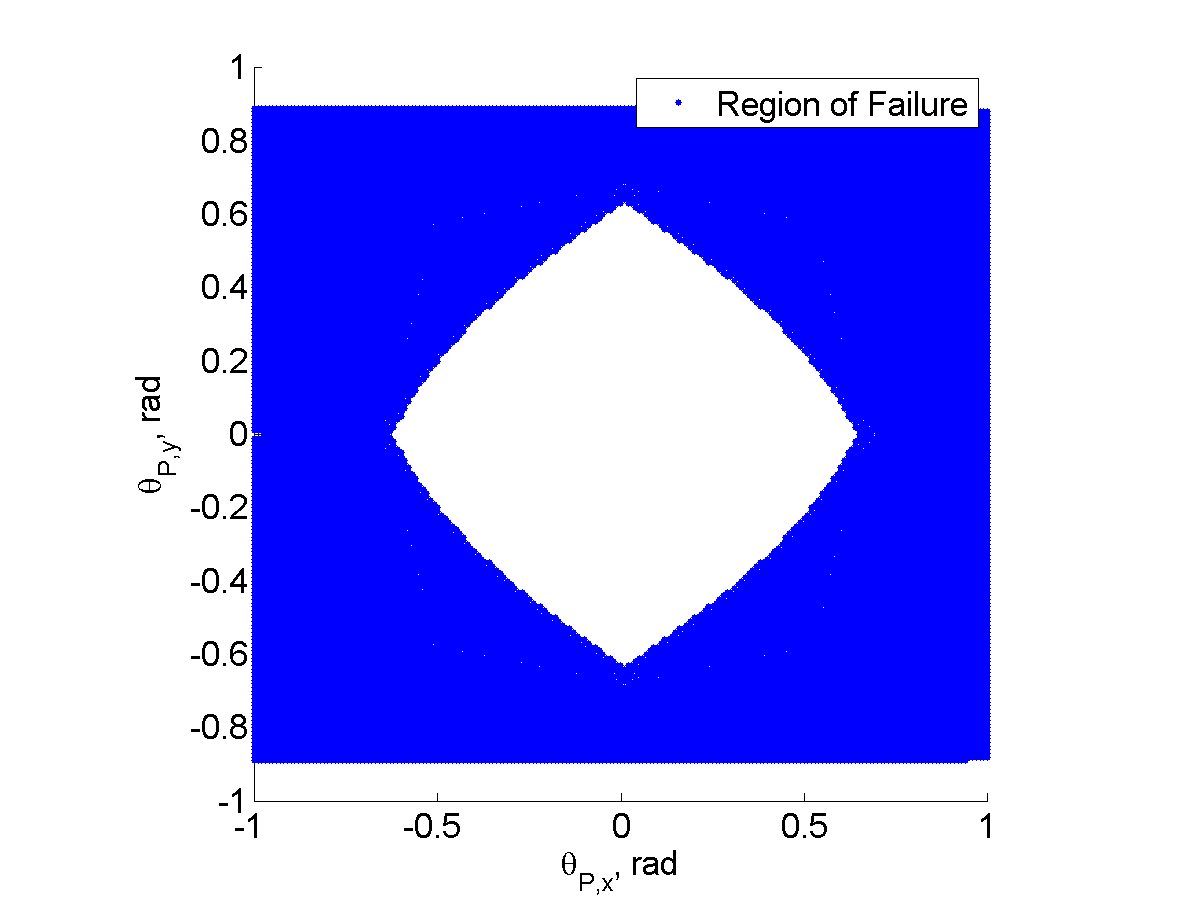
\includegraphics[width=0.495\textwidth]{ori_rom.png}}
				\caption{Range of motion for body's planar position (\emph{left}) and body pitch and roll (\emph{right}) while in the default stance.}
				\label{fig::pos_and_ori_rom}
			\end{figure}
			It can be seen from Figures \ref{fig::pos_and_ori_rom} that the platform can achieve a maximum pitch and roll of  $\pm37^o$and a total displacement of $\pm 1.4 \text{ cm}$ along the \emph{x} and \emph{y} axis of $O_{b'}$.


		\subsection{Velocity Kinematics}

			Using the DH-coordinate transformation, ${H}^{i,0}_{i,4}$, the velocity kinematics of each \Ith leg are derived as the Jacobian $J^{i,0}_{i,e} \InRe{6\times4}$ where 
				\begin{equation}
					\dot{x}^{i,0}_{i,e} = J^{i,0}_{i,e}  \dot{q}_{i}
					\label{eq::leg_jacobian}
				\end{equation}
			with $\dot{x}^{i,0}_{i,e} \InRe{6}$ being stacked vector of translational and rotational velocities, $\dot{p}_{i,e}^{i,0} \InRe{3}$ and $\dot{\theta}_{i,e}^{i,0}\InRe{3}$, respectively, of each \Ith foot with respect to frame $O_{i,0}$. The matrix $J^{i,0}_{i,e}$ is defined explicitly in Appendix \ref{appendix::a}.

			Assuming the translational and rotational velocity of the trunk, $\dot{p}_{b}$ and $\dot{\theta}_{b}$, respectively; and the translational and rotational of each \Ith foot, $\dot{p}_{i,e} \InRe{3}$ and $\dot{\theta}_{i,e} \InRe{3}$, respectively, are known, the translation velocity of each \Ith foot can be written with respect to frame $O_{i,0}$ by:
				\begin{equation}
					\dot{p}_{i,e}^{i,0} \equiv \wrap{R^{0}_{i,0}}^{T} \wrap{ \dot{p}_{i,e} - \dot{p}_{b} - \Skew{ \dot{\theta}_{b} } \wrap{ {p}_{i,e} - {p}_{b} - R^{0}_{i,0} \vec{o}_{\nu} } }
				\end{equation}
			where $\vec{o}_{\nu} = [\nu,0,0]^{T}$, $R^{0}_{i,0}$ is the rotation-matrix component of the transformation $H^{0}_{i,0}$ defined in \ref{eq::world_to_dh}, and $\Skew{*}$ is the standard skew-symmetric matrix operator, which takes a $3\times1$ vector input. The corresponding rotational velocity of each \Ith foot  can be computed with respect to $O_{i,0}$ by:
				\begin{equation}
					\Theta^{i,0} \equiv \wrap{ R^{0}_{i,0} }^{T} \Skew{ \dot{\theta}_{i,e} - \dot{\theta}_{b} } R^{0}_{i,0}  = \Skew{ \dot{\theta}^{i,0}_{i,e} }
				\label{eq::velocity_skew}
				\end{equation}
			where the rotational velocity of each foot, described by $\dot{\theta}^{i,0}_{i,e}$, is recovered by:
				\begin{equation}
					\dot{\theta}^{i,0}_{i,e} \equiv \sbrack{ 
						-\Theta^{i,0}_{1,2},
						 \Theta^{i,0}_{1,3},
						-\Theta^{i,0}_{2,3}
					}^{T}
				\end{equation}
			with $\Theta^{i,0}_{j,k}$ being the \Kth element in the \Jth row of the skew symmetric matrix $\Theta^{i,0}_{j,k}$ which results from \ref{eq::velocity_skew}.

			Joint velocities required to attain $\dot{x}^{i,0}_{i,e}$ can be computed using $J^{i,0}_{i,e}$. However, since each of BlueFoot's of legs had 4 degrees of freedom, $J^{i,0}_{i,e}$ is rank deficient and $\dot{q}_{i}$ cannot be obtained by direct inversion. Instead, $\dot{q}_{i}$ can be approximated from $\dot{x}^{i,0}_{i,e}$ by a weighted, Penrose-Moore psuedo-inverse of $J^{i,0}_{i,e}$, which is defined as follows:
				\begin{eqnarray}
					\dot{q}_{i} &\approx& \sbrack{J^{i,0}_{i,e}}_{\Lambda_{j}}^{\dagger} \dot{x}^{i,0}_{i,e} \nonumber \\
					\dot{q}_{i} &\approx& \wrap{ \wrap{J^{i,0}_{i,e}}^{T}J^{i,0}_{i,e} + \Lambda_{J} }^{-1} \wrap{J^{i,0}_{i,e}}^{T}\dot{x}^{i,0}_{i,e}
				\end{eqnarray}
			where $\Lambda_{J}$ is a strictly positive-definite weighting matrix that is typically chosen to have 
				\begin{equation*}
					\text{det}(\Lambda_{J}) \ll 1.
				\end{equation*}
			The operator $\sbrack{*}_{\Lambda_{j}}^{\dagger}$ defines a weighted pseudo-inversion off a matrix argument $(*)$ given a positive-definite weighting matrix $\Lambda_{j}$. A weighted pseudo-inversion is chosen over direct pseuedo-inversion to avoid a non-smooth set of solutions $\dot{q}_{i}$. Degenerate solutions for $\dot{q}_{i}$ exist at particular manipulator configurations where $\wrap{\wrap{J^{i,0}_{i,e}}^{T}J^{i,0}_{i,e}}$ is non-invertible.




	\section{Dynamical Model}
	

		\subsection{System State Vector and General-Form Dynamics}
		
			The dynamical model of the BlueFoot platform is treated a general, free-floating body with four ridged legs, each of which have four degrees of freedom. This system is fully described by the state vector $z \equiv [\eta^{T}, \dot{\eta}^{T}]^{T} \RealVec{44}$ and its dynamics are:
				\begin{equation}
					M(\eta)\ddot{\eta} + C(\eta,\dot{\eta})\dot{\eta} + G(\eta) + \Delta{H} = \tau + J^T(\eta) f_{ext} %
					\label{eq::normal_form_dynamics}
				\end{equation}
			where $M(\eta)$, $C(\eta,\dot{\eta}$), $G(\eta)$ and $J(\eta)$ represent the system mass matrix, Coriolis matrix, gravity matrix and Jacobian, respectively \cite{Wieber2006}. $\Delta{H}$ has been included as a lump term to account for dynamical uncertainties, such as friction or unmodeled coupling effects. Additionally, $f_{ext} = [ f_{1,ext}^{T},f_{2,ext}^{T},f_{3,ext}^{T},f_{4,ext}^{T}]^{T} \RealVec{24}$ represents a stacked vector of force-wrenches, $f_{i,ext} \RealVec{6}$, applied to the system through each \Ith foot. The state vector, $\eta$, can be partitioned as follows: $\eta = [ {p}_{b}^{T}, \theta_{b}^{T}, q^{T} ]^{T}$ with ${p}_{b} \RealVec{3}$ and $\theta_{b} \RealVec{3}$ representing the position and orientation, respectively, of the quadruped's trunk in an arbitrarily placed world coordinate frame, and $q \RealVec{16}$ is a vector of joint variables, $m$ of which are contributed by each leg. $\tau \RealVec{22}$ represents a vector of generalized torque inputs and takes the form $\tau = [ 0_{1x6}, \tau_{q}^{T} ]^{T}$ where $\tau_{q}$ represents a set of torque inputs to each joint. It is important to note that the states we are most interested in controlling, ${p}_{b}$ and $\theta_{b}$, are not directly actuated, and must be controlled via composite leg joint motions.		

			BlueFoot's dynamics, from \ref{eq::normal_form_dynamics}, can be realized in a general, compact, state-space form by:
				\begin{equation}
					\begin{split}
					\dot{z}_{1} 				&= z_{2} \\
					\dot{z}_{2} 				&= M^{-1}(z_{1})(\tau + \Phi(z_{1},z_{2},f_{ext})) \\
					\Phi(z_{1},z_{2},f_{ext}) 	&= J^T(z_{1}) f_{ext} - C(z_{1},z_{2})z_{2} - G(z_{1}) - \Delta{H}
					\end{split}
					\label{eq::state_space_dynamics}
				\end{equation}
			where $z_{1}=\eta$ and $z_{2}=\dot{\eta}$. The notation $\Phi(z_{1},z_{2},f_{ext})$ is introduced for convenience as a composite dynamical term. This term will be referred to, simply, as $\Phi$ in the sections that follow. The system dynamics are also considered in an approximate, discrete-time (first-order) form as follows:
				\begin{equation}
					\begin{split}
					{z}_{1,k+1} &= {z}_{1,k} + ( {e}_{1,k}^{\Delta_{s}} + {z}_{2,k} )\Delta_{s} \\
					{z}_{2,k+1} &= {z}_{2,k} + M^{-1}_{1,k}( {e}_{2,k}^{\Delta_{s}} + \tau_{k} + \Phi_{k}) \Delta_{s} \\
					t 			&= \Delta_{s} k
					\end{split}
					\label{eq::sampled_dynamics}
				\end{equation}
			where $M_{1,k} = M(z_{1,k})$ and $\Delta_{s} \equiv (f_{s})^{-1}$ with $f_{s}$ defining a uniform sampling frequency in Hz. The terms ${e}_{1,k}^{\Delta_{s}}$ and ${e}_{2,k}^{\Delta_{s}}$ are used to explicitly account for system discretization errors, which vary with respect to the step-size, $\Delta_{s}$. 

		\subsection{Joint-Servo Dynamics}

			The motor dynamics driving each joint need to be considered for use in control design since the input to BlueFoot's servo motors at each joint is a reference position command. In model-based control schemes to follow, a simple model of the motor dynamics will be utilized. Moreover, servos are considered as simple torque generators of the following form:
				\begin{equation}
					\tau_{q} = k_{s}(q^{r}-q)
					\label{eq::servo_control_dynamics}
				\end{equation}
			where $k_{s}>0$ is a constant, scalar gain and $q^{r}$ is a joint position reference. The servos being utilized to drive the leg joints of the BlueFoot quadruped have high-gain position feedback which allows us to model the motors, simply, as a static block which transform reference trajectories to torque outputs. All of these servos are identical, and thus have identical gains. One could instead consider the full motor dynamics for computing reference positions given a desired torque. The simple model stated above was adequate for achieving desired results with all proposed control schemes which use this torque-generator model.


		%\subsection{Single Leg Dynamics}
			
		%	The dynamics of each independent leg (with each base-frame fixed) can be derived in closed form. These dynamics have been included in Appendix [B] using the previously defined notations.


	\section{BlueFoot Simulator}

		\begin{figure}[h!]
			\centering
			\fbox{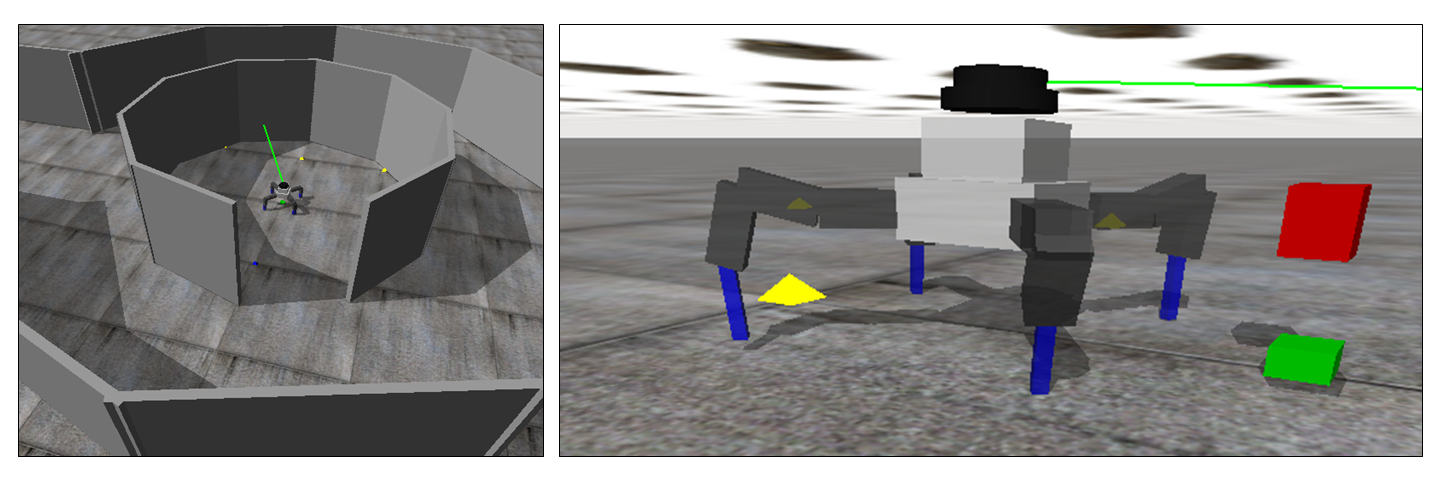
\includegraphics[width=1.00\textwidth]{simulation_wide_pic.png}}
			\caption{Visualization of the BlueFoot simulator.}
			\label{fig::simulator_wide}
		\end{figure}

		The BlueFoot platform is comprised of 17 rigid bodies, 16 of which are linkages between joints; and a main platform. Since each limb is formed from four revolute joints, the system has a total of 22 DOF, 16 of which are actuated. The main platform's configuration is generated through particular configurations of the legs. Furthermore, because each linkage is constrained to a rotation about a single axis, the rigid-body dynamic model of the BlueFoot quadruped is represented by 44 states. These states represent the position and velocity of each joint, $q_{i}$ and $\dot{q}_{i}$, respectively. Additionally, foot contact states are represented by binary scalars, $\mu_{i} \in \wrap{0,1}$, which describes whether the foot is not in contact or in contact, respectively.

		The dynamics of this system are somewhat complex because the quadruped's legs continuously make and break contact with the ground during gaiting. Additionally, the surface attributes and contact effects may vary significantly during gaiting and for various environments. A numerical dynamics engine, Open Dynamics Engine (ODE) \cite{ODE_Website}, has been utilized to implement a dynamics simulator for the BlueFoot platform. The simulator allows for various reconfigurations of environmental parameters, such as joint-friction, body-contact friction, and physical obstacles. Additionally, this simulation environment is implemented with a variety of geometric collision solvers and and efficient collision search method.

		The simulator's numerical engine, based on ODE is updated at 1000 Hz to attain high-fidelity, especially during contact phases, which require higher-than-normal integration stability to achieve reasonable  simulation accuracy. The input to the simulator is the desired main body configuration (i.e., position and orientation); desired foot placements; and desired ankle orientations, from which an inverse kinematic model is solved to attain all the desired joint configurations for the legs. Servos at each joint have built-in, tunable proportional controllers that effectively render them as ideal torque generators responding to the command input, as depicted in \ref{eq::servo_control_dynamics}. To mimic the behavior of the system, the commands to each joint motor are updated at 50 Hz, which matches the update rates at which the actual robot serves the P-controllers at each joint with reference positions. This rate has been chosen to account for the speed of inter-processor communications, and is adequate given the operating bandwidth of the robot.
		
		The BlueFoot simulator utilizes a dynamical model of the platform which consists of purely rectangular bodies. To match the dynamics of the true system, the individual mass and inertia parameters of each rigid body have been generated using a 3D model analysis software. This software takes into account geometric irregularities and variation of materials when computing the inertia of each body. The simulator also contains IMU and LIDAR sensor models for gathering feedback from the simulated environment. Each sensor is modeled with appropriate measurement noise so as to more closely match the performances of the actual IMU and LIDAR sensors on-board the BlueFoot platform.

			\begin{figure}[!h]
				\centering
				\fbox{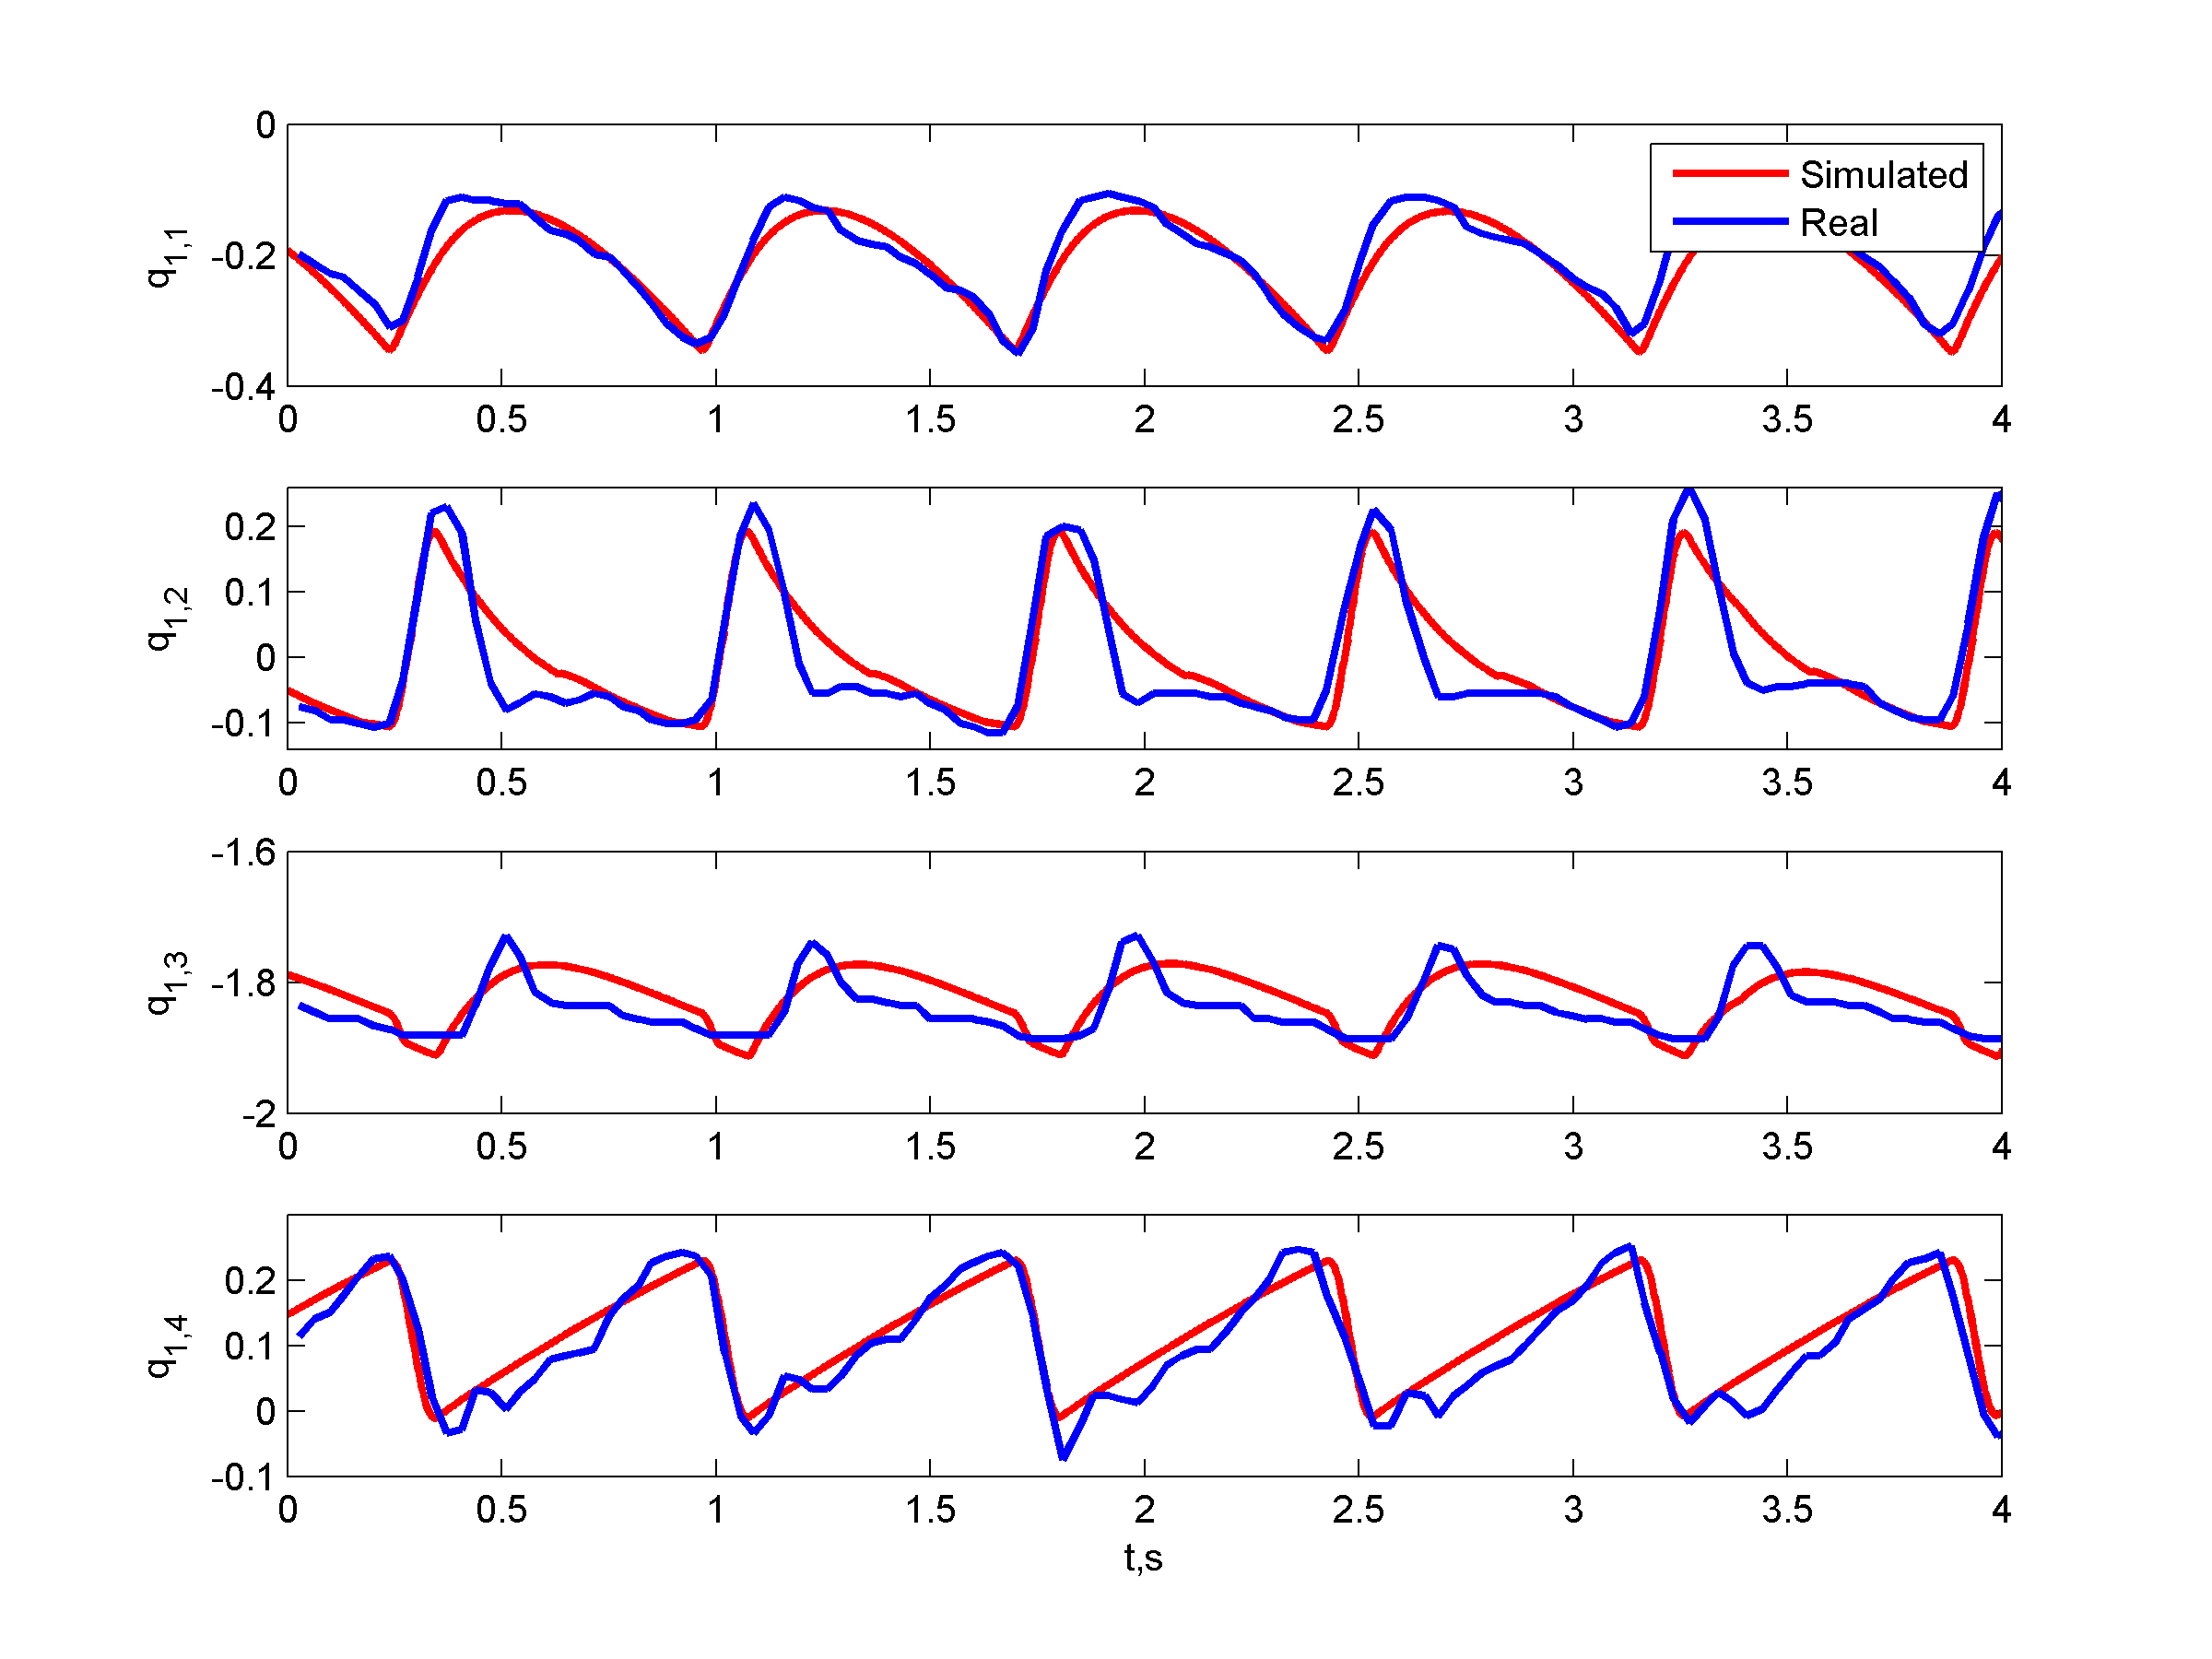
\includegraphics[width=1.00\textwidth]{sim_comparison.png}}
				\caption{Joint position comparison between the simulated and real quadruped while performing a gait which achieves a forward velocity of $60\frac{mm}{s}$}
				\label{fig::sim_performance_comparison}
			\end{figure}

		Careful, manual tuning was performed on simulated robot parameters, including joint update gains, joint-friction and surface-friction model coefficients to achieve closer matches between simulated results and the actual robot motions. A performance comparison can be seen in \ref{fig::sim_performance_comparison}, which shows joint position outputs for all joints of the front-right leg of the actual and simulated robot while performing a forward gait at $0.060$ m/s. It can be seen in  that the simulator provides and approximate representation true system performance within some margin of error. The discrepancies between the two data sets can be seen to usually occur at the minima of each series when the robot makes contact with the ground after a step. These differences can be attributed to ground-contact model inaccuracies. Work is still left to be done in improving the simulator's contact model, but this is more the fault of the simulation software libraries being used, namely in its low-order contact models. These contact models are very simplistic for the sake of simulation speed. Contact models could certainly be improved such that they more closely matches the effects of real-world surfaces. Additionally, discrepancies could also be attributed to the low-order joint model being used to represent the system's servo motors at each joint, described in \ref{eq::servo_control_dynamics}. This model neglects the effects of higher-order frictional effects which modify the rotation profile at each joint. All of the other simulated leg joints exhibited similar results to the actual motions.

		Despite these discrepancies, this simulation platform has proven to be adequate for use in testing gaiting and control algorithms which have been implemented on the real system. Moreover, all motion control algorithms which were first developed in this simulated environment have been ported to the real robot platform and performed in a highly comparable manner.

		The simulator has also been utilized to model BlueFoot's on-board LIDAR unit for use in testing navigation and terrain mapping algorithms and associated motion routines. Laser hits are modeled as force-less collisions between a ray-type geometry, used to represent the laser beam of the LIDAR, and environmental elements. Because the ray geometry can penetrate environmental elements in multiple places, or even multiple elements within the environment at a single instance, some post processing is performed on collision point returned by the simulator such that the point of intersection \emph{closest} to the robot is taken as a laser-beam hit. Additionally, sensor realism is imposed by limiting the data access frequency to buffered laser data by control routines operating the simulated robot to a rate of 10 Hz, which matches the scan rate of BlueFoot's on-board LIDAR. The angular velocity of the spinning laser head and the depth of each laser beam hit are corrupted by zero-mean Gaussian random noise with variances close to the parameters specified in the datasheet of the LIDAR unit.
